\documentclass[11pt]{article}
\usepackage{calc}
\usepackage[margin={1in,0.5in},footskip=0in]{geometry}
\usepackage[miniquiz]{hwk}
\usepackage{tikz}

\renewcommand{\theclass}{math 1300}
\renewcommand{\dateinfo}{September 25, 2012}
\renewcommand{\theassignment}{Quiz 3}

\begin{document}
\pagestyle{empty}
\newsavebox{\quizfront}
\begin{lrbox}{\quizfront}
\begin{minipage}[top][4.5in][t]{\textwidth} \setlength{\parindent}{1.5em}
\drawtitle
\vspace{-0.5in}
\begin{enumerate}

\item The graph below represents position $s$ of an object (in feet)
  as a function of time $t$ (in seconds).
  \vspace{-.35in}
  \begin{center}
    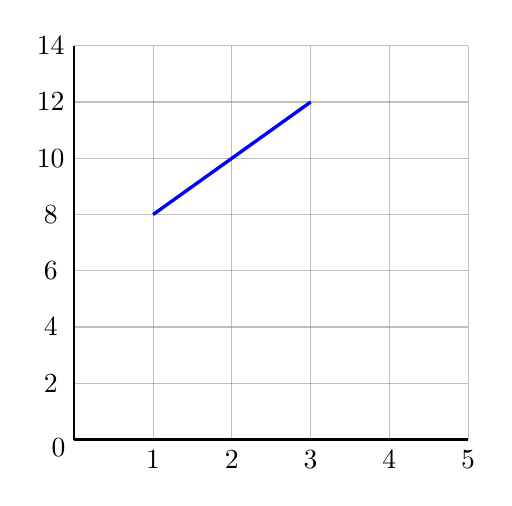
\begin{tikzpicture}[xscale = 1, yscale = 5/14]
      \def\xmin{0}\def\xmax{5} \def\ymin{0}\def\ymax{14} 
      \foreach \i in {\xmin,...,\xmax} {\ifnum\i=0{}
        \else{\draw[gray, thin, opacity=.5]
          (\i,\ymin) -- (\i,\ymax);\draw node at (\i, -.7) {$\i$};}\fi}
      \foreach \i in {2,4,6,8,10,12,14} {\ifnum\i=0{}
        \else{\draw[gray, thin, opacity=.5]
          (\xmin, \i) -- (\xmax, \i);\draw node at (-.3, \i) {$\i$};}\fi}
      \draw node at (-.2, -.3) {$0$};
      
      \draw[thick] (\xmin,0) -- (\xmax,0); \draw[thick] (0,\ymin) --
      (0,\ymax);
      
      \draw[very thick, domain=\xmin:\xmax, -] plot[samples=200]
      function{-2*x*(x-5)};
      \draw[very thick, blue] (1,8) -- (3,12);
    \end{tikzpicture}
  \end{center}
  \vspace{-.25in}
  Find the average velocity over the interval $[1,3]$. Include units.
  \vfill
  
  {\color{blue} The average velocity is $\dfrac{s(3)-s(1)}{3-1} =
    2\,\frac{\text{feet}}{\text{second}}$.}

  \vfill

\end{enumerate}
%\begin{flushright}
%\textsc{over} $\longrightarrow$
%\end{flushright}



\end{minipage}
\end{lrbox}

%%%%%%%%%%%%%%%%%%%%%%%%%%%%%%%%%%%%%%%%%%%%%%%%%%%%%%
%%%% This is for the back of the quiz
%%%%%%%%%%%%%%%%%%%%%%%%%%%%%%%%%%%%%%%%%%%%%%%%%%%%%%
\newsavebox{\quizback}
\begin{lrbox}{\quizback}
\begin{minipage}[top][4.5in][t]{\textwidth} \setlength{\parindent}{1.5em}
\begin{itemize}
\item[2.] If $f(x) = x^2 + 5x + 1$, find the average rate of change of
  $f$ on $[0,2]$.

  \vfill
  {\color{blue}
    The average rate of change is $\dfrac{f(2)-f(0)}{2-0} = 7$.
  }
  \vfill


\end{itemize}
\end{minipage}
\end{lrbox}

%%%%%%%%%%%%%%%%%%%%%%%%%%%%%%%%%%%%%%%%%%%%%%%%%%%%%%
%%%%
%%%% Now we make two copies of the ``quizfront'' box
%%%%
%%%%%%%%%%%%%%%%%%%%%%%%%%%%%%%%%%%%%%%%%%%%%%%%%%%%%%%
\noindent \usebox{\quizfront}
\vfill
\noindent \usebox{\quizback}

%%%% Uncomment the rest to have a two-sided quiz.
%\pagebreak
%\noindent \usebox{\quizback}
%\vfill
%\noindent \usebox{\quizback}
\end{document}